\section{Technique}
\label{sec:technique}

In this section, we formalize our technique for reasoning about movement within a coarse `unit cube' space.
Starting from spatial traces, we map sequences of positions into both occupied cubes as well as nodes in a graph, then discuss three classes of properties: individual actor properties, multiple actor properties, and properties of paths.

\subsection{Foundations and Definitions}
We begin with a set of time-sequenced traces $\mathcal{T}$ of spatial data, with an individual trace $T\in\mathcal{T} = (t,x,y,z)$ where $t\in\mathbb{R}$ is a time relative to a global start time, and $x,y,z\in \mathbb{R}$ are familiar position co-ordinates relative to a world frame. 
We assume all traces share identical time and world frames, or they have been synchronized by pre-processing.
Let trace $T$ be indexed by $i$ so that $T_i$ is the $i$th time-ordered record in $T$, and let the set of traces $\mathcal{T}$ be indexed so $T^i$ is the $i$th trace in $\mathcal{T}$. 

Each trace pertains to an \emph{actor}, designated collectively as the set $\mathsf{A}$ and individually as $\bigstar$. 
The relation $\mathsf{B}$ links an actor $\bigstar^i$ to trace $T^i$.


Let there exist a space $Cube^3 \equiv \mathbb{Z}^3$.  In this space we denote a function $f_{cube}$ that maps from a trace record to a cube, $f_{cube} : T_i \rightarrow cube_i$. 


\begin{equation}
f_{cube}(t,x,y,z) = (\lfloor \alpha * x \rfloor, \lfloor \alpha * y \rfloor , \lfloor \alpha * z \rfloor )
\label{eq:fcube}
\end{equation}

The symbol $\alpha$ in Eq.~\ref{eq:fcube} denotes a scaling factor to convert between the original unit of measure to the size of the unit cube (See Sec.~\ref{sec:observations} for a discussion of choosing the size of the unit cube).
For each record in a trace $T$, we both map its position to a cube and add a node to a multigraph $G = (V,E)$, if it does not already exist. $G$ can be thought of as embedded within $Cube^3$.

\begin{equation}
  cube_i \Rightarrow v_i \in V
\end{equation}

Cubes and nodes in $G$ are in a one-to-one correspondence within a relation $R$.

If a trace $T$ contains two consecutive records $T_i$ and $T_{i+1}$ that map to different cubes, then we add an edge $(v_i, v_{i+1})$ to $E$. 
Every edge is assigned a label of the time $t$ from $T_{i+1}$ with a label function $w$, so that the edge label indicates the time when the $cube_i$ transitioned to $cube_{i+1}$.
For every edge $e\in E$ we associate a predecessor and successor, identified in relations $F_{prev}$ and $F_{next}$, denoted collectively as $\mathsf{F}$.

\begin{equation}
  \left( f_{cube}(T_i) \neq f_{cube}(T_{i+1}) \right) \Rightarrow (v_i, v_{i+1}) \in E
\end{equation}

We denote a path between vertices $v_i$ and $v_j$ by $P(v_i, v_j)$ and consider this notation equivalent:

\begin{equation}
  P(v_i, v_j) \equiv P(cube_i, cube_j)
\end{equation}

A spatial abstraction, then, is the tuple:

\begin{equation}
\cube = (\mathcal{T}, \mathsf{A}, \mathsf{G}, \mathsf{R}, Cube^3, \mathsf{F}, \mathsf{B}, w)
\end{equation}

%, where $\mathbb{T}$ is a set of traces, $G$ is a directed multigraph, $R$ is a relation mapping $cube_i$ to graph node $v_i$, $C^3$ is the unit cube space, $F$ is the successor relation mapping edges in $G$ to their successors, and $A$ is a relation mapping actor $\bigstar_i$ to trace $T$.


%Let the $i$th element of the trace file be designated $\T_i$, and to the position data in $\bigstar_i$ we apply $f_{\cube}$ and infer the existence of cube $\cube_i$.

%$$\bigstar_i \Rightarrow (\cube_i | \cube_{xyz\in \mathbb{N}} = f_{\cube}(\bigstar_{xyz})$$ 

%This maps every record in the trace file to a cube.
%Simultaneously, we create a root node $v_i$ in a directed multigraph $G = (V,E)$.
%For each subsequence trace record $\bigstar_{i+1}$, we check if this position maps to the same cube, $\cube_i$, or to a new cube, $\cube_{j}.$
%If a record maps to a new cube $\cube_{j}$, then we add a directed edge to $E$ from $v_i$ to $v_{j}$.  
%We add a label the edge $(v_i, v_j)$ with the time $t$.
%The node $v_i$ corresponds to $\cube_i$ and the node $v_{j}$ corresponds to $\cube_{j}$.
%From the existence of this edge we say there is a path from $\cube_i$ to $\cube_j$ denoted $\cube_{i\rightsquigarrow j}$.  More formally,

A property, $\phi$ is said to be true for a spatial abstraction $\cube$ if the definition of $\phi$ holds for $(\mathcal{T}, \mathsf{A}, \mathsf{G}, \mathsf{R}, Cube^3, \mathsf{F}, \mathsf{B}, w)$.
We denote this by 

\begin{equation}
  \cube \models \phi
\end{equation}

And say a spatial abstraction ``models" $\phi$.
One spatial abstraction can model multiple properties, and properties can pertain to particular actors, groups of actors, paths, or cubes.
A list of properties is presented in tabular form below.

\subsection{Properties of Single Actors}

\emph{Note: all properties in this table pertain to a particular actor $\bigstar^i$.}
\begin{tabular}{| p{2.8cm} | p{11.5cm} | }
\hline
PROPERTY & FORMALISM \\ \hline
% Move to multiple places & $\phi_{\{multiplePlaces\}} = \exists (P(b_{home}, b_a), P(b_{home}, b_b)| b_a \neq b_a)$ \\ \hline
Moves & $\phi_{\{moves\}} = |V| > 1$ \\ \hline
Returns Home & $\phi_{\{returnhome\}} = \exists P(cube_{home}, cube_{home})$ \\ \hline
No repetition & $\phi_{\{noRepetition\}} = \forall (v_a, v_b), (v_c,v_d) in E, v_b \neq v_c, v_a \neq v_d$ \\ \hline
 Loiters & $\phi_{\{loiters\}} =  \exists e \in E$ s.t. $e[time] - e_{prev}[time] > k$; $k$ is time bound \\ \hline
Teleports & $\phi_{\{teleport\}}=  \exists  cube_i, cube_j | (F_{next}(cube_i, cube_j) \land \lnot Adjacent(cube_i, cube_j))$ \\ \hline
Hot Box & $\phi_{\{hotBoxOfSizeN\}} = \exists b_i, v_i \in E | n \geq |\{e \in E | e(v_x, v_i), v_x \in E\}$ \\ \hline
\end{tabular}

Informally, the above properties correspond to the following descriptions.
``Moves" checks whether the actor visits any cube other than its initial one.
``Returns home" check whether the actor leaves the initial cube and returns to it at a later point in time.
``No repetition" checks that an actor does not re-enter some cube after leaving it.
``Loiters" checks that an actor does not stay in some cube for longer than some given time bound.
``Teleports" checks that the cube trace is connected within the cube-map, meaning there are no ``skipped," or vacant cubes between successive time steps.
``Hot box" checks if any cube in the map has been visited at least a specified number of times.


\subsection{Properties of Multiple Actors}
\begin{tabular}{| p{2.8cm} | p{11.5cm} | }
\hline
PROPERTY & DEFINITION \\ \hline
 Independence& $\phi_{\{independence\}} =  \forall V_{\bigstar_i},V_{\bigstar_j} \in V, i \neq j \rightarrow V_{\bigstar_i} \cap V_{\bigstar_j} = \emptyset $ \\ \hline
  $k$-independence& $\phi_{\{k-independence\}} =  \forall V_{\bigstar_i},V_{\bigstar_j} \in V, i \neq j \rightarrow V_{\bigstar_i} \cap V_{\bigstar_j} = \emptyset $ \\ \hline
 Following & $\phi_{\{following\}} =  \exists E' \subset E_1 \land E'' \subset E_2$ s.t. $P(E')=P(E'') $  \\ \hline
 Dense Space & $\phi_{\{dense\}} = \exists S \subset Cube^3$ s.t. $> k \bigstar$'s occupy $S$ at time $t$\\ \hline
 Sparse Space & $\phi_{\{sparse\}} = \exists S \subset Cube^3$ s.t. $< k \bigstar$'s occupy $S$ at time $t$\\ \hline
 Slow Traffic& $\phi_{\{slowTraffic\}} = \exists S \subset Cube^3$ s.t. $> \forall \bigstar \in S \phi_{\{loiters>k\}}$ \\ \hline
 Fast Traffic & $\phi_{\{fastTraffic\}} = \exists S \subset Cube^3$ s.t. $> \forall \bigstar \in S \phi_{\{loiters<k\}}$ \\ \hline
 Mobbing& $\phi_{\{mobbing\}} = \exists [t_i, t_j] \land S \subset Cube^3$ s.t. $ \phi{\{dense\}}(t_i) < \phi{\{dense\}}(t_j)$ \\ \hline
 Fleeing& $\phi_{\{fleeing\}} = \exists [t_i, t_j] \land S \subset Cube^3$ s.t. $ \phi{\{dense\}}(t_i) > \phi{\{dense\}}(t_j)$ \\ \hline
 SConnected& $\phi_{\{SConnected\}} = \exists SCC \in E$ \\ \hline
% not sure how to do these formulas in a nice way with graphs yet
% these are only for two entities
 Above & $\phi_{\{above\}} =  T^1_i[z] > T^2_i[z] \forall i$ where $i$ is indexing a time interval\\ \hline
 Below & $\phi_{\{below\}} = T^1_i[z] < T^2_i[z]  \forall i$ where $i$ is indexing a time interval\\ \hline
 Front & $\phi_{\{front\}} = T^1_i[x] > T^2_i[x]  \forall i$ where $i$ is indexing a time interval\\ \hline
 Behind & $\phi_{\{behind\}} = T^1_i[x] < T^2_i[x]  \forall i$ where $i$ is indexing a time interval\\ \hline
 Right & $\phi_{\{right\}} = T^1_i[y] > T^2_i[y]  \forall i$ where $i$ is indexing a time interval \\ \hline
 Left & $\phi_{\{left\}} = T^1_i[y] < T^2_i[y]  \forall i$ where $i$ is indexing a time interval \\ \hline
\end{tabular}

Informally, the above properties correspond to the following descriptions.
``Independence" checks that any two actors never occupy the same cube at any point in a trace.
``Following" checks to see if any two actors share a given cube-path at any point in a trace.
``Dense" checks to see if many actors occupy some subspace of $Cube^3$ at a given time.
``Sparse" checks to see if relatively few actors occupy some subspace of $Cube^3$ at a given time.
``Slow Traffic" identifies a subspace where the time difference of all successive edges is greater than a value $k$. 
``Fast Traffic" identifies a subspace where the time difference of all successive edges is less than a value $k$. 
``Mobbing" identifies a time window during which a subspace has more actors entering that leaving. 
``Fleeing" identifies a time window during which a subspace has more actors leaving than entering. 
``SConnected" identifies a strongly connected component (SCC) in the graph.
Collectively, SCCs partition $Cube^3$ into disconnected subspaces.
This property can hold for one or more actors.
The ``above/below" and remaining properties specify partial order properties corresponding to the six directions in \rthree for some time-interval within a trace.

\subsection{Properties of Paths}
\subsubsection{The Ratio Cube}

\begin{wrapfigure}{l}{0.3\textwidth}
  \centering
    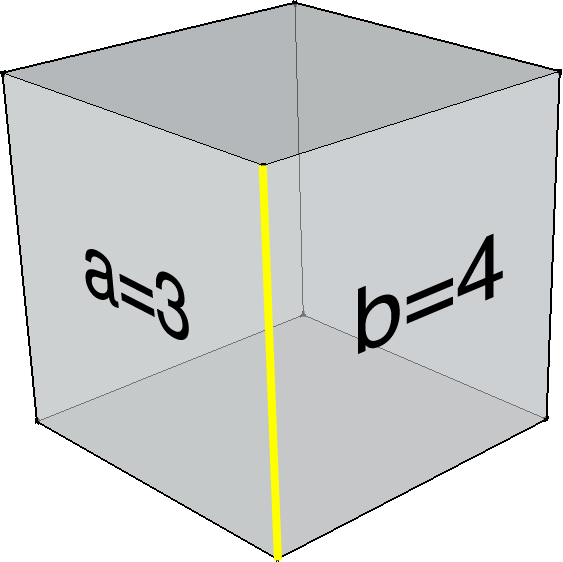
\includegraphics[width=0.3\textwidth]{./figures/ratioCube_3_4}
      \caption{The ratio cube.}
      \label{fig:ratioCube}
\end{wrapfigure}
In order to compare multiple paths, we consider for each path $P$ a method of counting how many times an actor moves in each direction.  
In our model, there are six directions: up, down, left, right, forward, back, and we assign a counter to each.
We then compare the ratios of the counters, and use this ratio as a way of comparing multiple paths.
A visual representation of these counters and the ratio between directions is shown in Fig.~\ref{fig:ratioCube}, and shows an example where a $P(cube_i, cube_j)$ moves in direction $a$ three units and direction $b$ four units.

As shown in the figure, the number of moves in each direction is associated with a face of the ratio cube, and the ratios between the directions is associated with an edge of the cube, depicted by a yellow line.


Figs.~\ref{fig:3by4}-\ref{fig:6by8} show ratio equivalent paths, that is, the ratio of the number of moves made in each of the six directions is the same.
Note than these ratios are invariant under transformation by scale.
Fig.~\ref{fig:6by8_squiggle} depicts a path that makes the same ratio of moves in a different order, and therefore all paths with identical ratios in the edge cube are likewise path ratio equivalent.


\begin{figure}
\centering
  \begin{minipage}[t]{.45\textwidth}
  \centering
  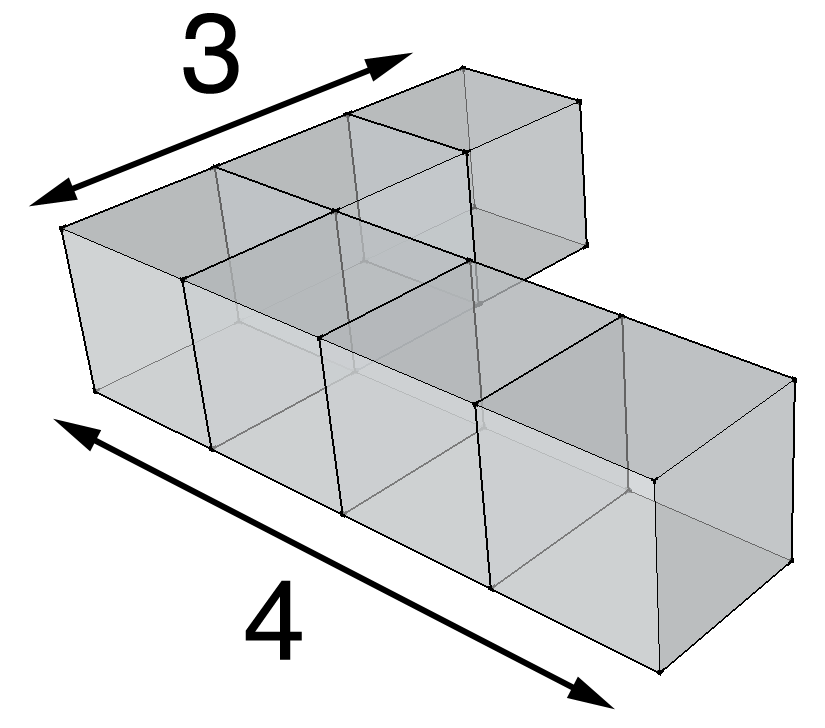
\includegraphics[width=0.9\textwidth]{./figures/3by4}
    \caption{A path with ratio $a:b = 3:4$}
		\label{fig:3by4}
  \end{minipage}
  \begin{minipage}[t]{.45\textwidth}
  \centering
  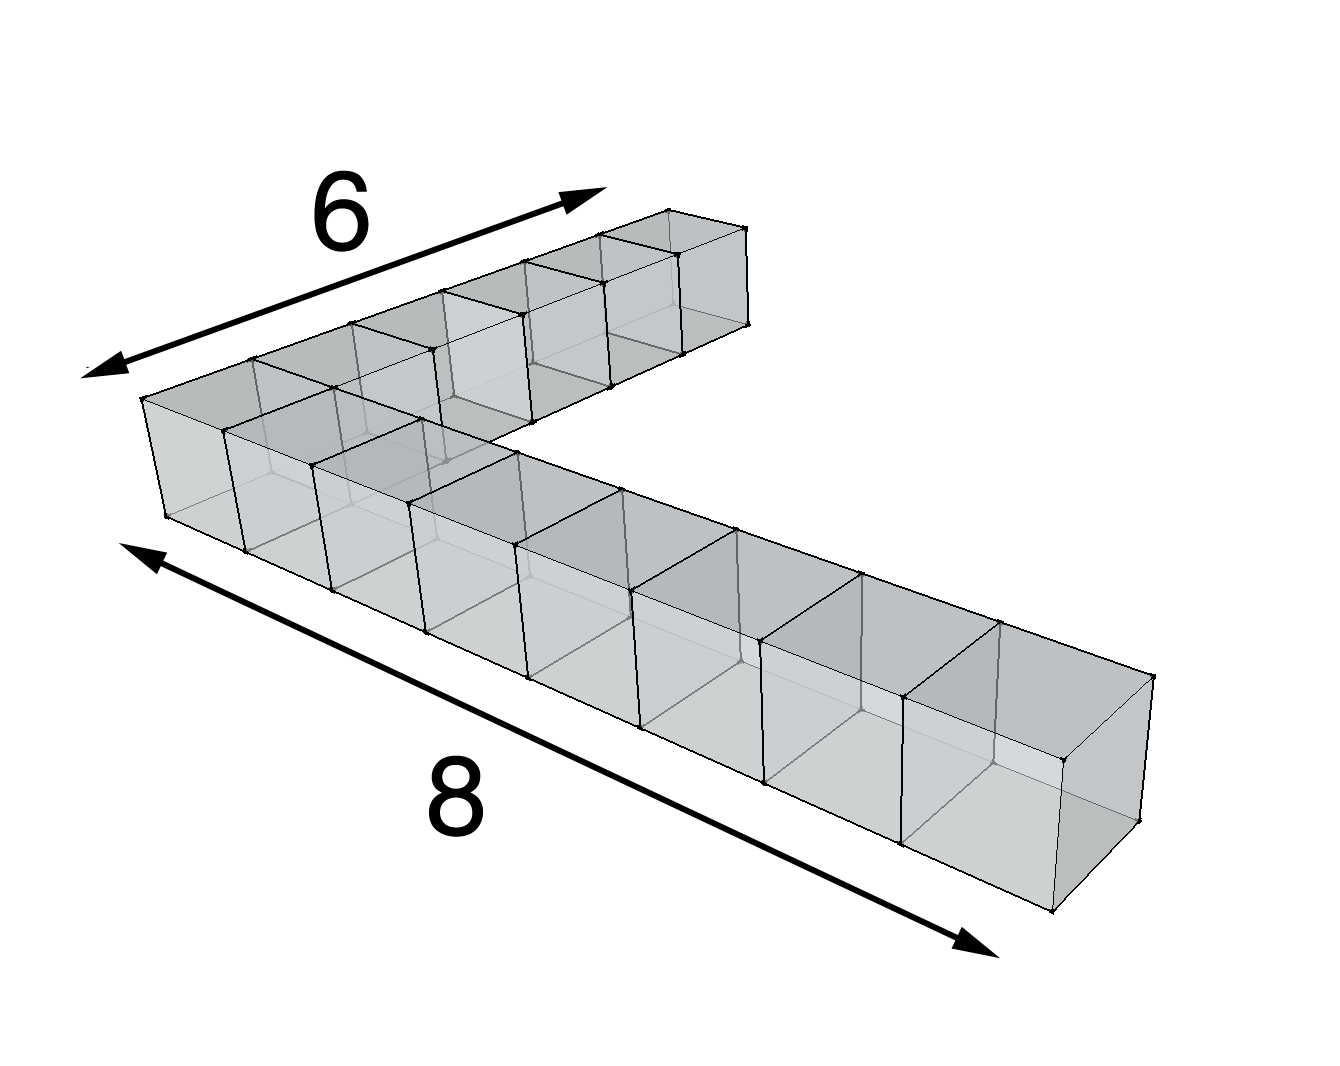
\includegraphics[width=0.9\textwidth]{./figures/6by8}
    \caption{Another path with ratio $a:b = 3:4$}
    \label{fig:6by8}
  \end{minipage}\hfill
  \begin{minipage}[t]{.45\textwidth}
  \centering
  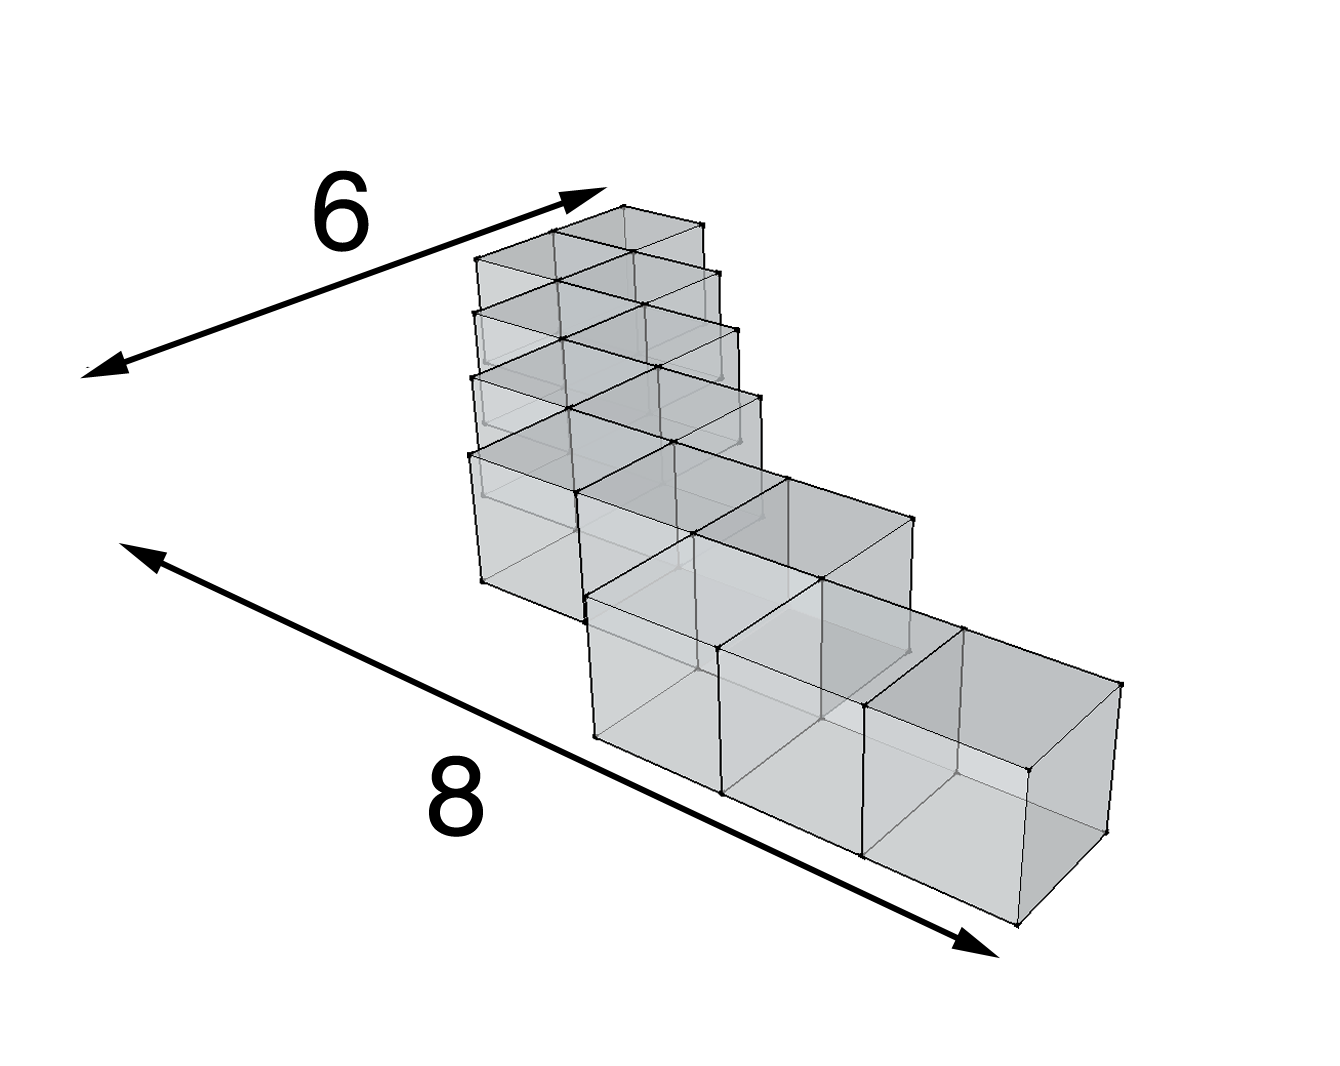
\includegraphics[width=0.9\textwidth]{./figures/6by8_squiggle}
    \caption{Alternate path also with ratio $a:b = 3:4$}
		\label{fig:6by8_squiggle}
  \end{minipage}
  \begin{minipage}[t]{.45\textwidth}
  \centering
  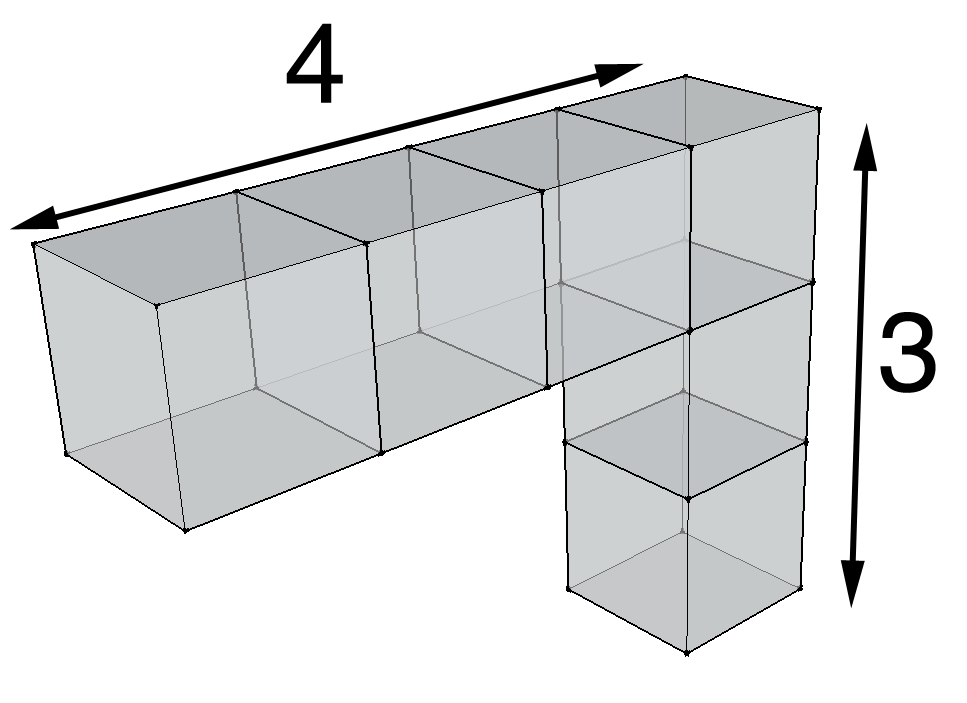
\includegraphics[width=0.9\textwidth]{./figures/3by4_upended.png}
  \caption{Path that after rotational transformation has ratio $a:b=3:4$} 
  \label{fig:3by4_upended}
  \end{minipage}\hfill
\end{figure}

    
An interesting case is exhibited in Fig.~\ref{fig:3by4_upended}, where the ratio is the same but along another edge.
We consider this path to be \emph{rotationally} ratio equivalent to the paths in Figs.\ref{fig:3by4}-\ref{fig:6by8_squiggle}a.
There are 24 rotational symmetries for a cube (one is the identity), so searching for ratio equivalence given two paths is tractable.

Cube ratios can also be useful for measuring the similarity of paths.
If the edge ratio is not identical but approximately the same, the two paths are \emph{approximately} edge ratio equivalent, to the extent of the measure of the difference of their ratios.



%Method:
%\begin{itemize}
 %\item partition space into boxes
 %\item enumerate the boxes
 %\item map a concrete positional trace through space onto its uniquely corresponding boxes
 %\item sync time frames of box-traces to infer spatio-temporal properties
 %\item using the spatio-temporal box-trace, derive properties (given elsewhere)
%\end{itemize}

%\emph{Selecting appropriate box size}

%Different box sizes may generate very different properties.

%\emph{Too small of a box} If you choose the boxes to be relatively small, the trace may show a teleport, which we define as a spatially disconnected box-trace.
%If there are gaps of disconnected boxes, and two entities collide in the unaccounted for space, the violation of box-independence will not be inferred.

%\emph{Too big of a box} If you choose the boxes to be relatively large, this may be too rough of an over approximation.
%For an extreme example, an entity never registers "leaving home" if its initial box is the size of the given dimensions.
%Sometimes large over-approximations are desired, such as if you only want to examine the movements across two ``hemispheres" of an entity's space.
